% =====================================================================
\chapter{Phương pháp nghiên cứu}
\label{chap:phuongphap}

Chương này trình bày cách đề tài trả lời ba câu hỏi nghiên cứu. Sau khi nhắc lại mục đích, câu hỏi và các điểm chính của tổng quan, chương mô tả khung nghiên cứu. Khung này gồm thiết kế thực nghiệm có đối chứng, cách xây dựng mô hình DACL, phân tích các thành phần mất mát, lựa chọn trọng số và cài đặt các phương pháp đối chứng. Hai mục cuối mô tả dữ liệu được thu thập và cách phân tích dữ liệu để trả lời từng câu hỏi.

\section{Mục đích nghiên cứu}

Như đã nêu ở Chương~\ref{chap:gioithieu}, đề tài xây dựng và đánh giá một mô hình phân đoạn tế bào máu dựa trên khung DACL khi dữ liệu có nhãn khan hiếm. Mô hình được so sánh với các phương pháp bán giám sát tiêu biểu trong cùng điều kiện. Đồng thời, đề tài phân tích cơ chế của các thành phần mất mát để lựa chọn cấu hình phù hợp cho ảnh hiển vi.

\section{Câu hỏi nghiên cứu}

\begin{enumerate}[label=\textbf{CH\arabic*.},leftmargin=1.6cm]
  \item DACL đạt độ chính xác như thế nào so với tám phương pháp bán giám sát và so với học có giám sát, ở mức 5\% và 10\% ảnh có nhãn?
  \item Lợi ích của DACL thể hiện ở loại lỗi nào và tập trung ở những ảnh nào?
  \item Các thành phần mất mát của DACL tương tác với nhau như thế nào, và cần chọn trọng số ra sao để huấn luyện ổn định khi mỗi vòng lặp chỉ có một ảnh có nhãn?
\end{enumerate}

\section{Tóm tắt tổng quan tài liệu}

Chương~\ref{chap:tongquan} cho thấy ảnh tế bào máu có nhiều đối tượng nhỏ, ranh giới mảnh giữa các tế bào chạm nhau và màu nhuộm biến thiên mạnh. Các phương pháp bán giám sát hiện có đi từ ràng buộc nhất quán trên một mạng đến đồng huấn luyện hai mạng dị thể, và tất cả đều phải cân bằng giữa việc khai thác nhãn giả và nguy cơ thiên lệch xác nhận. DACL bổ sung một ràng buộc đồng thuận trên toàn bộ phân phối xác suất của hai mạng. Hiệu quả của khung này trên ảnh hiển vi, cũng như cách các thành phần mất mát tương tác với nhau khi tín hiệu giám sát yếu, là những điểm đề tài cần làm rõ.

\section{Khung nghiên cứu}

\subsection{Thiết kế thực nghiệm có đối chứng}

Đề tài sử dụng thiết kế thực nghiệm có đối chứng. Biến độc lập là phương pháp huấn luyện, gồm mười một mô hình: UNeXt và Swin-Unet học có giám sát, tám phương pháp bán giám sát đối chứng, và DACL. Biến phụ thuộc là bốn độ đo chất lượng phân đoạn trên từng ảnh kiểm thử. Các yếu tố được giữ cố định cho mọi phương pháp gồm cách chia dữ liệu, tiền xử lý, tăng cường dữ liệu, bộ tối ưu, lịch tốc độ học, số vòng huấn luyện, cách chọn mô hình theo tập kiểm định và cách tính độ đo. Toàn bộ mười một mô hình được xây dựng lại từ đầu bằng PyTorch trong cùng một khung mã, dưới dạng các notebook tự chứa chỉ khác nhau ở ô cấu hình và hàm mất mát (Phụ lục~\ref{app:code}). Nhờ đó, khác biệt về kết quả có thể quy cho thuật toán thay vì cho điều kiện thí nghiệm.

\subsection{Xây dựng mô hình DACL}
\label{sec:dacl-impl}

Mô hình được xây dựng dựa trên mô tả kiến trúc và hàm mất mát của khung DACL~\cite{wang2026dacl}, gồm UNeXt, Swin-Unet, giáo viên EMA của Swin-Unet và hàm mục tiêu~\eqref{eq:total}. Bảng~\ref{tab:dacl-config} tóm tắt cấu hình huấn luyện mà đề tài sử dụng.

\begin{table}[ht]
\centering
\caption{Cấu hình huấn luyện mô hình DACL của đề tài.}
\label{tab:dacl-config}
\small
\begin{tabularx}{\textwidth}{>{\raggedright\arraybackslash}p{4.4cm} >{\raggedright\arraybackslash}X}
\toprule
Thành phần & Cấu hình \\
\midrule
Kích thước đầu vào & $224\times224$ \\
Thời lượng huấn luyện & 30\,000 vòng lặp \\
Bộ tối ưu & SGD, tốc độ học 0,01 giảm theo đa thức bậc 0,9; momentum 0,9; weight decay $10^{-4}$ \\
Lô dữ liệu & 1 ảnh có nhãn + 4 ảnh không nhãn \\
Khởi tạo Swin-Unet & Swin-T tiền huấn luyện trên ImageNet-1K \\
Trọng số $\{\lambda,\tau,\beta\}$ & $\{0{,}2;\,0{,}2;\,1\}$ (mục~\ref{sec:weights}) \\
Ramp-up trọng số & Sigmoid trong 12\,000 vòng đầu \\
Hệ số EMA của giáo viên & 0,99 \\
Ghép cặp cho $\Lict$ & $\sigma=0{,}5$; hai nửa của lô 4 ảnh không nhãn \\
Dạng của $\Lict$ & Trung bình bình phương sai khác trên bản đồ xác suất \\
Phạm vi của $\Ldac$ & Ảnh không nhãn; gradient qua cả hai mạng \\
Giáo viên khi sinh mục tiêu & Chế độ suy luận, tắt stochastic depth \\
Tăng cường dữ liệu & Chỉ ảnh có nhãn (Bảng~\ref{tab:aug}) \\
Chọn mô hình & DSC kiểm định của UNeXt, đánh giá mỗi 500 vòng lặp \\
\bottomrule
\end{tabularx}
\end{table}

Kích thước đầu vào $224\times224$ và thời lượng 30\,000 vòng lặp được chọn để vừa với tài nguyên tính toán, vì phải huấn luyện mười một mô hình ở nhiều mức nhãn. Hai thông số này áp dụng như nhau cho mọi phương pháp. Đầu vào $224\times224$ cũng khớp với độ phân giải mà trọng số Swin-T được tiền huấn luyện. Với 30\,000 vòng lặp và 884 ảnh không nhãn ở mức 5\%, mỗi ảnh không nhãn được duyệt qua khoảng 136 lần.

Một số chi tiết cài đặt cần được xác định cụ thể. $\Lict$ được tính trên bản đồ xác suất softmax và lấy trung bình theo điểm ảnh, như cách làm phổ biến của ICT~\cite{verma2022ict}. $\Ldac$ được tính trên ảnh không nhãn, giống phạm vi của $\Lcps$, và gradient của nó lan truyền qua cả hai mạng. Lô bốn ảnh không nhãn được chia thành hai nửa để ghép cặp trộn. Giáo viên EMA được đặt ở chế độ suy luận khi sinh mục tiêu. Lý do là Swin-Unet trong đề tài dùng stochastic depth~\cite{huang2016stochdepth} với tỷ lệ 0,1. Nếu giáo viên giữ chế độ huấn luyện, mục tiêu nội suy sẽ thay đổi ngẫu nhiên giữa các lần gọi, trái với vai trò cung cấp mục tiêu ổn định của mô hình giáo viên.

\subsection{Phân tích các thành phần mất mát của DACL}
\label{sec:loss-analysis}

Mục này là phân tích của đề tài, nhằm trả lời phần đầu của câu hỏi CH3. Thay hệ thức~\eqref{eq:jsd} vào~\eqref{eq:lent}, số hạng entropy tại mỗi điểm ảnh có thể viết lại thành
\begin{equation}
  H(p)+H(q)-H\big(\tfrac{p+q}{2}\big)=\tfrac12\big[H(p)+H(q)\big]-\JSD(p,q).
  \label{eq:lent-decomp}
\end{equation}
Hệ thức này cho thấy $\Lent$ chứa hai tác động ngược chiều. Thành phần $\tfrac12[H(p)+H(q)]$ là cực tiểu hóa entropy theo nghĩa của Grandvalet và Bengio~\cite{grandvalet2005entropy}, tức là đẩy mỗi mạng về dự đoán tự tin. Thành phần $-\JSD(p,q)$ lại thưởng cho sự \emph{khác biệt} giữa hai mạng. Nếu xét riêng $\Lent$, giá trị nhỏ nhất đạt được khi hai mạng tự tin tuyệt đối nhưng trái ngược nhau. Chẳng hạn, với $p=(1,0)$ và $q=(0,1)$, cả hai entropy bằng 0, còn JSD đạt cực đại $\log 2$. Khi đó $\Lent=-\log 2$, là giá trị nhỏ nhất có thể có. Như vậy, tác dụng khuyến khích đồng thuận của $\Ldac$ không đến từ $\Lent$, mà đến từ $\Lkl$.

Ví dụ số làm rõ sự cân bằng giữa hai số hạng. Xét bài toán hai lớp và xác suất lớp tế bào của hai mạng tại một điểm ảnh. Khi hai mạng cùng dự đoán $0{,}9$, ta có $\Lkl=0$ và $\Lent=H(0{,}9)\approx0{,}325$. Khi hai mạng dự đoán lần lượt $0{,}99$ và $0{,}6$, $\Lent$ giảm xuống $\approx0{,}222$, nhưng $\Lkl\approx0{,}459$ nên tổng $\Ldac\approx0{,}681$. Tổng $\Ldac$ do đó vẫn ưu tiên sự đồng thuận, nhờ số hạng KL. Tuy nhiên, khi hai mạng đã đồng thuận ($p=q$), $\Lkl$ bằng 0 và $\Lent$ trở thành $H(p)$. Toàn bộ $\beta\Ldac$ khi đó tác động như một số hạng cực tiểu hóa entropy với hệ số $\beta$, áp lên mọi điểm ảnh của ảnh không nhãn.

Hệ quả của phân tích này là trong DACL có ba cơ chế cùng đẩy hai mạng về những dự đoán tự tin: nhãn giả cứng của $\Lcps$, thành phần entropy của $\Lent$, và sự đồng thuận do $\Lkl$ áp đặt. Khi hai mạng đã cùng sai ở một vùng, cả ba cơ chế đều củng cố lỗi đó thay vì sửa nó. Đây đúng là điều kiện để thiên lệch xác nhận xuất hiện~\cite{arazo2020pseudo}. Mức độ rủi ro phụ thuộc trực tiếp vào độ lớn của $\lambda$ và $\beta$ so với tín hiệu giám sát thật, nên việc lựa chọn trọng số được xem xét riêng ở mục tiếp theo.

\subsection{Lựa chọn trọng số các thành phần mất mát}
\label{sec:weights}

Đề tài sử dụng bộ trọng số $\{\lambda,\tau,\beta\}=\{0{,}2;\,0{,}2;\,1\}$. Bộ trọng số này được chọn dựa trên bốn căn cứ sau.

\paragraph{Tương quan giữa ba thành phần không giám sát.} Trọng số của $\Ldac$ được đặt lớn gấp năm lần trọng số của $\Lcps$ và $\Lict$, theo tỷ lệ $\lambda:\tau:\beta=1:1:5$ của cấu hình tham khảo trong~\cite{wang2026dacl}. Tỷ lệ này đặt trọng tâm vào ràng buộc đồng thuận kép, là thành phần đặc trưng của khung DACL, trong khi vẫn giữ giám sát chéo và nhất quán nội suy ở vai trò bổ trợ.

\paragraph{Cân bằng với tín hiệu giám sát khi chỉ có một ảnh có nhãn.} Độ lớn của các số hạng có thể đọc trực tiếp từ log huấn luyện. Ở vòng lặp thứ 100 với 5\% nhãn, khi các mạng chưa học được nhiều, ta có $\Lsup\approx0{,}96$ (tổng của hai mạng), $\Lcps\approx0{,}98$, $\Lict\approx0{,}050$ và $\Ldac\approx0{,}35$. Với bộ trọng số của đề tài ở giá trị đầy đủ, phần không giám sát bằng $0{,}2\times0{,}98+0{,}2\times0{,}05+0{,}35\approx0{,}56$, tức khoảng 0,58 lần phần có giám sát. Nếu tăng cả ba trọng số lên mười lần, phần này sẽ bằng khoảng 5,6, tức gấp 5,8 lần phần có giám sát. Ở vòng 10\,000, khi hệ số ramp-up là 0,87, các số hạng đã giảm còn $\Lsup\approx0{,}42$, $\Lcps\approx0{,}15$, $\Lict\approx0{,}028$ và $\Ldac\approx0{,}070$. Phần không giám sát sau khi nhân trọng số khi đó bằng khoảng 0,09, tức 22\% phần có giám sát. Với trọng số lớn hơn mười lần, tỷ lệ này sẽ là khoảng 2,2 lần. Do lô chỉ có một ảnh có nhãn, tín hiệu giám sát thật ở mỗi vòng lặp vốn đã nhiễu. Khi phần không giám sát lớn gấp nhiều lần phần có giám sát, gradient chủ yếu đến từ việc hai mạng học theo nhau. Theo phân tích ở mục~\ref{sec:loss-analysis}, đó chính là điều kiện để lỗi chung được củng cố. Bộ trọng số $\{0{,}2;\,0{,}2;\,1\}$ giữ phần có giám sát ở vai trò chủ đạo trong suốt quá trình huấn luyện.

\paragraph{Thống nhất bậc độ lớn với các phương pháp đối chứng.} Các phương pháp đối chứng dùng trọng số nhất quán tối đa 0,1, là giá trị mặc định của SSL4MIS~\cite{luo2020ssl4mis}. Với $\lambda=0{,}2$ áp lên tổng hai số hạng giám sát chéo, mỗi mạng trong DACL nhận trọng số giám sát chéo cùng bậc với CPS và CTCT. Nhờ đó, so sánh trở nên công bằng hơn: khác biệt về kết quả phản ánh cấu trúc của hàm mất mát, thay vì cường độ của nó.

\paragraph{Kết quả thử nghiệm sơ bộ.} Ở bước thử nghiệm sơ bộ, đề tài đã thử bộ trọng số lớn hơn mười lần, $\{2;\,2;\,10\}$, là cấu hình được sử dụng trong~\cite{wang2026dacl}. Lần thử này dùng cùng thiết lập, ở mức 5\% nhãn, và giáo viên còn để ở chế độ huấn luyện. Huấn luyện không ổn định: khi hệ số ramp-up vượt khoảng 0,65, DSC kiểm định của UNeXt giảm từ 0,93 xuống khoảng 0,83 và không hồi phục. Cùng lúc đó, DSC kiểm định của hai mạng trở nên gần như trùng nhau, phù hợp với kịch bản hai mạng hội tụ về cùng một lời giải sai.

Bộ trọng số được xác định theo các căn cứ trên trước khi chạy các thí nghiệm chính. Đề tài không dò tìm siêu tham số và không dùng tập kiểm thử để chọn trọng số. Trọng số không giám sát của DACL, cũng như của mọi phương pháp đối chứng, tăng dần theo ramp-up sigmoid~\cite{laine2017temporal} trong 12\,000 vòng đầu, tức 40\% thời lượng huấn luyện.

\subsection{Cài đặt các phương pháp đối chứng}
\label{sec:baseline-impl}

Các phương pháp không dựa trên cặp CNN--Transformer dùng mạng UNeXt, còn các phương pháp CNN--Transformer dùng cặp UNeXt và Swin-Unet. Trong mọi trường hợp, mạng UNeXt là mạng được đánh giá, nên mọi phương pháp có cùng chi phí suy luận. Bảng~\ref{tab:baselines} tóm tắt cách cài đặt. Trọng số của từng phương pháp được lấy theo công bố hoặc mã nguồn của chính phương pháp đó khi có thông tin; nếu không có, đề tài dùng giá trị mặc định 0,1 của SSL4MIS. Ba phương pháp được điều chỉnh để phù hợp với khung thí nghiệm chung. Với PCPCS, mạng Mamba của Semi-Mamba-UNet được thay bằng Swin-Unet, để mọi phương pháp CNN--Transformer dùng chung một cặp mạng. Với DSTCT, cặp U-Net và ViT cũng được thay bằng UNeXt và Swin-Unet vì cùng lý do. Với LMCT, thành phần đối sánh InfoNCE không được đưa vào. Công bố của phương pháp này không định nghĩa cặp mẫu dương và âm, và trong mã nguồn công khai, giá trị của thành phần này được tách khỏi đồ thị tính toán nên không tạo ra gradient.

\begin{table}[ht]
\centering
\caption{Cài đặt các phương pháp bán giám sát. Mọi trọng số không giám sát (trừ $\lambda_{con}$ của PCPCS) tăng theo ramp-up sigmoid trong 12\,000 vòng đầu.}
\label{tab:baselines}
\footnotesize
\begin{tabularx}{\textwidth}{>{\raggedright\arraybackslash}p{1.4cm} >{\raggedright\arraybackslash}p{3.2cm} >{\raggedright\arraybackslash}X >{\raggedright\arraybackslash}p{2.6cm}}
\toprule
Phương pháp & Mạng & Thành phần không giám sát & Trọng số tối đa \\
\midrule
MT & UNeXt + giáo viên EMA (0,99) & MSE giữa xác suất của học sinh và giáo viên; đầu vào giáo viên có nhiễu Gauss độ lệch chuẩn 0,1 & 0,1 \\
DCT & 2 UNeXt & JSD giữa hai mạng; mất mát khác biệt góc nhìn với ví dụ đối kháng FGSM, $\epsilon=0{,}02$ & $\lambda_{cot}=10$; $\lambda_{dif}=0{,}5$ \\
CPS & 2 UNeXt & CE + Dice với nhãn giả cứng của mạng kia & 0,1 \\
ICT & UNeXt + giáo viên EMA (0,99) & MSE trên ảnh trộn, $\lambda\sim\mathrm{Beta}(0{,}2;0{,}2)$, hai nửa lô không nhãn & 0,1 \\
CTCT & UNeXt + Swin-Unet & Dice với nhãn giả cứng; $\Lsup$ lấy trung bình hai mạng & 0,1 \\
PCPCS & UNeXt + Swin-Unet & Dice với nhãn giả cứng; MSE giữa đầu ra của hai mạng sau gộp trung bình toàn cục và chuẩn hóa L2 & 0,1; $\lambda_{con}=1$ \\
DSTCT & UNeXt + Swin-Unet + giáo viên EMA của Swin-Unet & Nhãn cứng (Dice); nhãn mềm làm sắc với nhiệt độ 0,1; chênh lệch độ quyết đoán; nhất quán với giáo viên & $\alpha=0{,}5$; $\beta=1$; $\gamma=3$; $\mu=0{,}1$ \\
LMCT & UNeXt + Swin-Unet & Dice với bản đồ xác suất mềm của mạng kia & 0,1 \\
DACL & UNeXt + Swin-Unet + giáo viên EMA (0,99) của Swin-Unet & $\Lcps$, $\Lict$, $\Ldac$ (mục~\ref{sec:lit-dacl}) & $\lambda=0{,}2$; $\tau=0{,}2$; $\beta=1$ \\
\bottomrule
\end{tabularx}
\end{table}

\subsection{Độ phức tạp mô hình}
\label{sec:complexity}

Số tham số và số phép tính của hai mạng được đo trên bản cài đặt của đề tài với đầu vào $224\times224$ (Bảng~\ref{tab:complexity}). Số phép tính được đếm bằng công cụ đếm FLOPs của PyTorch, trong đó một phép nhân--cộng được tính là hai FLOPs. UNeXt với cấu hình kênh $\{32,64,128,160,256\}$ có 1,58 triệu tham số, nhỏ hơn Swin-Unet khoảng 17 lần. Mọi phương pháp bán giám sát đều triển khai bằng UNeXt, nên chi phí suy luận của chúng giống hệt nhau, và khác biệt chỉ nằm ở chi phí huấn luyện.

\begin{table}[ht]
\centering
\caption{Độ phức tạp của hai mạng ở đầu vào $224\times224$.}
\label{tab:complexity}
\small
\begin{tabular}{lccc}
\toprule
Mạng & Tham số (triệu) & GFLOPs & Vai trò trong DACL \\
\midrule
UNeXt $\{32,64,128,160,256\}$ & 1,58 & 1,80 & Huấn luyện và suy luận \\
Swin-Unet tiny & 27,17 & 12,15 & Chỉ huấn luyện \\
\bottomrule
\end{tabular}
\end{table}

\section{Thu thập dữ liệu}
\label{sec:setup}

\subsection{Bộ dữ liệu}
\label{sec:dataset}

Đề tài sử dụng bộ dữ liệu Blood Cell Segmentation do Depto và cộng sự công bố~\cite{depto2021blood}, phân phối qua kho mã nguồn theo giấy phép MIT~\cite{depto2021repo}. Kho mã mô tả đây là bộ dữ liệu phân đoạn tế bào máu hiển vi lớn nhất tại thời điểm công bố, gồm 1\,328 ảnh gốc và 1\,328 mặt nạ chuẩn. Đây là nhận định của nhóm tác giả bộ dữ liệu, đề tài không tự kiểm chứng. Trang mã nguồn không mô tả nguồn gốc tiêu bản, thiết bị chụp, loại thuốc nhuộm, loại tế bào được gán nhãn hay quy trình gán nhãn. Vì vậy, các đặc điểm dưới đây là kết quả đo đạc trực tiếp trên dữ liệu đã tải về.

Toàn bộ 1\,328 ảnh đều ghép được với mặt nạ cùng tên. Có 1\,209 ảnh định dạng PNG và 119 ảnh JPEG, còn mọi mặt nạ đều là PNG. Về độ phân giải, 1\,208 ảnh có kích thước $1600\times1200$ điểm ảnh và 120 ảnh có kích thước $1944\times1383$, gợi ý rằng ảnh được thu từ ít nhất hai cấu hình chụp khác nhau. Kiểm tra 60 mặt nạ đầu tiên cho thấy mỗi mặt nạ chỉ chứa hai mức xám, tức là mặt nạ nhị phân. Ở độ phân giải $640\times480$, điểm ảnh thuộc tế bào chiếm trung bình 29,4\% diện tích ảnh, dao động từ 4,2\% đến 73,2\%. Số vùng liên thông (lân cận 8) trong một mặt nạ có trung bình 58,5, trung vị 56, thấp nhất 8 và cao nhất 169. Số vùng liên thông là cận dưới của số tế bào, vì các tế bào có khe tách bị đứt được tính chung thành một vùng.

\begin{figure}[ht]
  \centering
  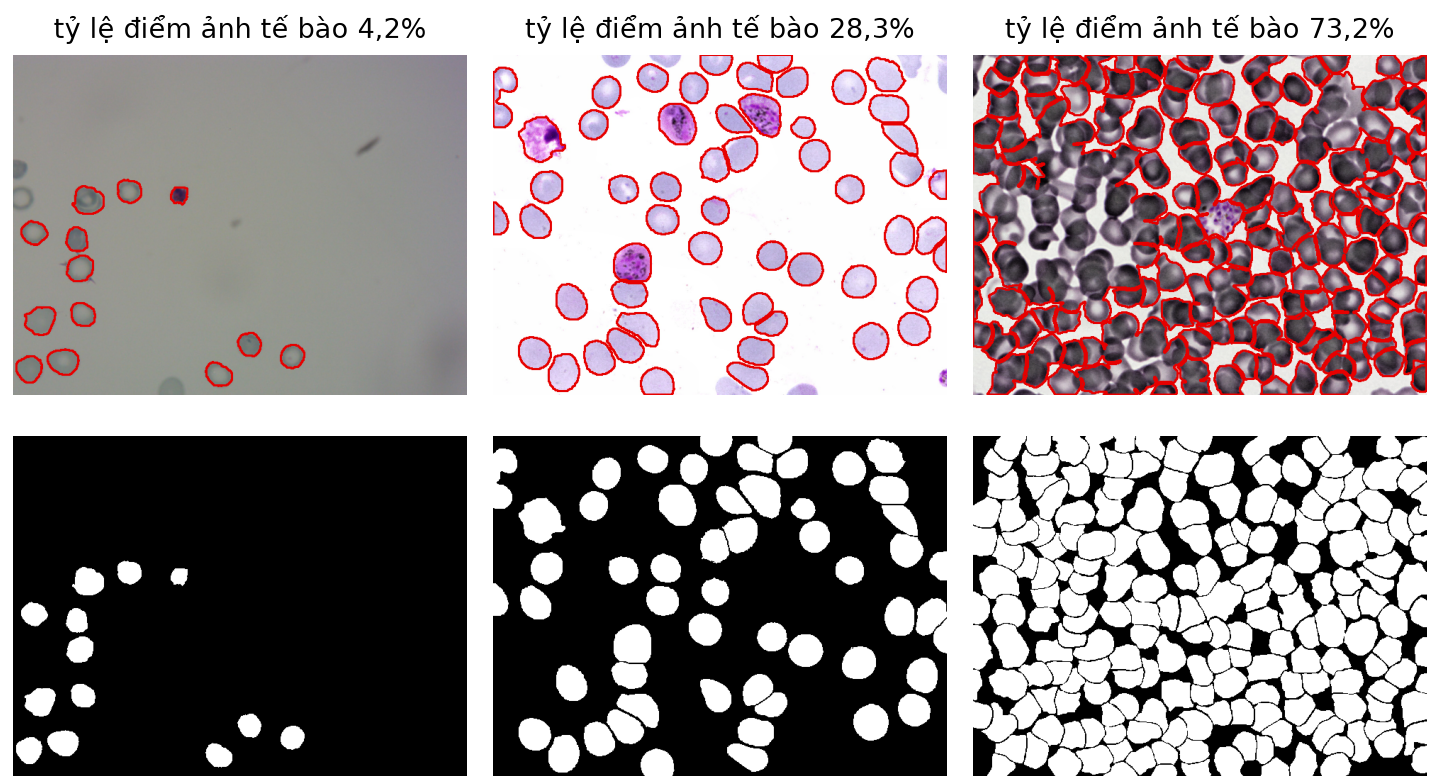
\includegraphics[width=\textwidth]{dataset_examples.png}
  \caption{Ba ảnh trong bộ dữ liệu có tỷ lệ điểm ảnh tế bào thấp nhất, ở mức trung vị và cao nhất. Hàng trên: ảnh gốc với đường viền mặt nạ chuẩn (màu đỏ). Hàng dưới: mặt nạ nhị phân. Ảnh đã được thu nhỏ về $640\times480$.}
  \label{fig:dataset}
\end{figure}

Hình~\ref{fig:dataset} cho phép rút ra ba quan sát. Một là, ba ảnh có nền và tông màu rất khác nhau, phù hợp với nhận định về độ biến thiên màu ở Chương~\ref{chap:tongquan}. Hai là, những tế bào có vùng bắt màu tím đậm ở ảnh giữa được gán cùng lớp với các tế bào còn lại, nên mặt nạ không phân biệt loại tế bào. Ba là, ở ảnh có mật độ cao, các tế bào chạm nhau được tách bằng các đường nền rất mảnh. Khi ảnh được thu nhỏ về $224\times224$ để đưa vào mạng, nhiều đường tách này bị mất. Vì vậy, sai số có xu hướng tập trung ở vùng tiếp giáp giữa các tế bào.

\subsection{Tiền xử lý và phân chia dữ liệu}

Ảnh được thu nhỏ một lần về $640\times480$, dùng nội suy theo diện tích cho ảnh và nội suy láng giềng gần nhất cho mặt nạ. Mặt nạ sau đó được nhị phân hóa với ngưỡng 127. Dữ liệu được xáo trộn với hạt giống cố định 2026 rồi chia theo tỷ lệ 70/10/20 thành tập huấn luyện, kiểm định và kiểm thử (Bảng~\ref{tab:split}). Các tập con có nhãn được lấy từ đầu danh sách huấn luyện đã xáo trộn, nên tập 5\% nằm trọn trong tập 10\%, và tập 10\% nằm trọn trong tập 20\%. Phần còn lại của tập huấn luyện được dùng như ảnh không nhãn: mặt nạ của chúng có trên đĩa nhưng không bao giờ được đọc khi huấn luyện. Khi đưa vào mạng, ảnh được thu nhỏ tiếp về $224\times224$, không giữ tỷ lệ khung hình $4:3$, và chuẩn hóa theo thống kê của ImageNet do Swin-Unet được tiền huấn luyện trên ImageNet~\cite{deng2009imagenet}.

\begin{table}[ht]
\centering
\caption{Phân chia dữ liệu. Tập kiểm định và kiểm thử giống nhau ở mọi tỷ lệ nhãn.}
\label{tab:split}
\small
\begin{tabular}{lcccc}
\toprule
Tập & Số ảnh & 5\% nhãn & 10\% nhãn & 20\% nhãn \\
\midrule
Huấn luyện (có nhãn / không nhãn) & 930 & 46 / 884 & 93 / 837 & 186 / 744 \\
Kiểm định                          & 133 & \multicolumn{3}{c}{133} \\
Kiểm thử                           & 265 & \multicolumn{3}{c}{265} \\
\midrule
Tổng                               & 1\,328 & & & \\
\bottomrule
\end{tabular}
\end{table}

\subsection{Tăng cường dữ liệu}

Tăng cường dữ liệu được thực hiện trực tuyến và chỉ áp dụng cho ảnh có nhãn. Ảnh không nhãn, ảnh kiểm định và ảnh kiểm thử chỉ được thu nhỏ và chuẩn hóa. Bảng~\ref{tab:aug} liệt kê các phép biến đổi. Nhóm hình học áp dụng đồng thời lên ảnh và mặt nạ, còn nhóm màu và chất lượng ảnh chỉ áp dụng lên ảnh. Phép biến thiên nhuộm trong không gian HED~\cite{tellez2018hed} vốn được thiết kế cho ảnh mô bệnh học nhuộm H\&E. Đề tài dùng nó như một xấp xỉ cho sự thay đổi cường độ thuốc nhuộm giữa các tiêu bản máu, với biên độ nhỏ để tránh làm bạc màu nền.

\begin{table}[ht]
\centering
\caption{Các phép tăng cường dữ liệu cho ảnh có nhãn ($p$: xác suất áp dụng).}
\label{tab:aug}
\small
\begin{tabularx}{\textwidth}{>{\raggedright\arraybackslash}p{2.6cm} >{\raggedright\arraybackslash}p{4.4cm} >{\raggedright\arraybackslash}X}
\toprule
Nhóm & Phép biến đổi & Tham số \\
\midrule
Hình học & Lật ngang, lật dọc, xoay $90^\circ$ & $p=0{,}5$ mỗi phép \\
         & Biến đổi affine & $p=0{,}5$; tỷ lệ $0{,}85$--$1{,}15$; xoay $\pm15^\circ$; dịch $\pm5\%$ \\
         & Biến dạng đàn hồi & $p=0{,}2$; $\alpha=30$, $\sigma=6$ \\
Màu và nhuộm & Color jitter & $p=0{,}5$; độ sáng, tương phản, bão hòa $\pm20\%$; sắc độ $\pm0{,}05$ \\
             & Biến thiên nhuộm HED & $p=0{,}5$; hệ số nhân $U(0{,}95;1{,}05)$; độ dịch $U(-0{,}005;0{,}005)$ \\
             & Gamma; CLAHE & $p=0{,}2$, $\gamma\in[0{,}8;1{,}2]$; $p=0{,}1$ \\
Chất lượng ảnh & Làm mờ Gauss; nhiễu Gauss & $p=0{,}1$, nhân $3$--$5$; $p=0{,}1$, độ lệch chuẩn $0{,}01$--$0{,}04$ \\
\bottomrule
\end{tabularx}
\end{table}

\subsection{Huấn luyện và thu nhận kết quả}

Mọi mô hình được huấn luyện 30\,000 vòng lặp bằng SGD với tốc độ học ban đầu 0,01, momentum 0,9 và weight decay $10^{-4}$. Tốc độ học giảm theo đa thức $\mathrm{lr}_t=0{,}01\,(1-t/30\,000)^{0{,}9}$~\cite{chen2018deeplab}. Huấn luyện dùng độ chính xác hỗn hợp FP16~\cite{micikevicius2018amp} trên GPU của nền tảng Kaggle. Mô hình học có giám sát dùng lô 8 ảnh có nhãn. Các phương pháp bán giám sát dùng lô gồm 1 ảnh có nhãn và 4 ảnh không nhãn, ghép thành một lần lan truyền xuôi. Cứ sau 500 vòng lặp, mô hình UNeXt được đánh giá bằng DSC trung bình trên tập kiểm định. Trọng số cho DSC kiểm định cao nhất được giữ lại và chỉ được đánh giá một lần trên tập kiểm thử. Mỗi cấu hình được huấn luyện một lần với hạt giống 2026.

Mỗi lần huấn luyện tạo ra ba loại dữ liệu phục vụ ba câu hỏi nghiên cứu. Bốn độ đo trên từng ảnh kiểm thử là dữ liệu chính cho CH1. Trọng số mô hình tốt nhất cho phép tính lại dự đoán trên từng ảnh, từ đó tính các đại lượng về loại lỗi cho CH2. Log huấn luyện ghi giá trị từng số hạng mất mát sau mỗi 100 vòng và DSC kiểm định sau mỗi 500 vòng, là dữ liệu cho CH3.

\section{Phân tích dữ liệu}

\subsection{Tính các độ đo}

Dự đoán được lấy theo lớp có xác suất lớn nhất và so sánh với mặt nạ ở độ phân giải $224\times224$. Biên của mặt nạ là tập điểm ảnh bị loại bỏ khi co mặt nạ bằng phần tử cấu trúc chữ thập $3\times3$. HD95 và ASD được tính theo đơn vị điểm ảnh ở độ phân giải này. Chúng không quy đổi được sang đơn vị vật lý, vì bộ dữ liệu không cung cấp kích thước thực của điểm ảnh. Kết quả được báo cáo dưới dạng trung bình (độ lệch chuẩn) trên 265 ảnh kiểm thử.

\subsection{Kiểm định thống kê (CH1)}

Vì mỗi phương pháp chỉ được huấn luyện một lần, khác biệt giữa DACL và từng mô hình khác được kiểm định bằng phép kiểm định hạng có dấu Wilcoxon~\cite{wilcoxon1945} trên cặp DSC của từng ảnh kiểm thử. Phép kiểm định này không giả định phân phối chuẩn, phù hợp với phân phối lệch của điểm số theo ảnh. Do DACL được so sánh với mười mô hình, ngưỡng ý nghĩa được hiệu chỉnh theo Bonferroni~\cite{dunn1961} thành $0{,}05/10=0{,}005$. Cách làm tương tự được áp dụng cho HD95 khi phân tích độ chính xác biên. Phép kiểm định này chỉ phản ánh sự biến thiên giữa các ảnh. Nó không tính đến dao động khi huấn luyện lại với hạt giống khác.

\subsection{Phân tích loại lỗi và độ khó của ảnh (CH2)}
\label{sec:analysis-rq2}

Để biết lợi ích của DACL đến từ loại lỗi nào, tất cả mô hình được chạy lại trên tập kiểm thử. Từ đó, đề tài tính độ chính xác (precision), độ phủ (recall) và tỷ lệ giữa diện tích dự đoán với diện tích mặt nạ chuẩn trên từng ảnh. Để biết lợi ích tập trung ở những ảnh nào, các ảnh kiểm thử được chia thành bốn nhóm theo tứ phân vị DSC của UNeXt học có giám sát, rồi so sánh hiệu DSC trong từng nhóm. Phần định tính dùng bốn ảnh có độ lệch chuẩn DSC giữa các mô hình lớn nhất. Tiêu chí khách quan này tránh việc chọn ảnh có lợi cho một phương pháp cụ thể.

\subsection{Phân tích diễn biến huấn luyện (CH3)}

Bên cạnh phân tích lý thuyết ở mục~\ref{sec:loss-analysis} và~\ref{sec:weights}, độ ổn định của DACL được đánh giá qua đường DSC kiểm định theo vòng lặp. Đường của DACL được so sánh với UNeXt học có giám sát và với hai phương pháp đối chứng tiêu biểu. Độ ổn định ở giai đoạn cuối được đo bằng trung bình và độ lệch chuẩn của DSC kiểm định trong 10\,000 vòng cuối.

Chương này đã mô tả khung nghiên cứu, gồm cách xây dựng mô hình DACL, phân tích các thành phần mất mát và căn cứ lựa chọn trọng số, cùng cách thu thập và phân tích dữ liệu cho từng câu hỏi nghiên cứu. Chương~\ref{chap:ketqua} trình bày các kết quả thu được, còn Chương~\ref{chap:ketluan} tóm tắt, rút ra kết luận và thảo luận ý nghĩa của chúng.
